\label{sec:results}
The table below illustrates the lowest classification errors we were able to achieve with our Decision Tree and LDA classifiers on the MNIST and Yale Extended B datasets. In LDA, we split the datasets in half so we can the other half for test. Using decision trees on MNIST, we utilized half of the dataset for training and half for testing. However, since the Yale B dataset is so small, we were only able to get lower error rates by using $\sim$95\% of the set for training and $\sim$5\% for testing (on decision trees.) For extra-trees, we split the two datasets in half to achieve our results.

\begin{table}[H]
  \centering
  \begin{tabular}{||c | c | c||} 
    \hline
    Algorithm & MNIST & Yale B \\
    \hline\hline
    LDA & 13.5\%  & 6.8\% \\ 
    \hline
    Decision Tree & 17.42\% & 57.89\% \\ 
    \hline
    Extra-Trees & 4.89\% (100 extra-trees) & 34.96\% (100 extra-trees) \\
    \hline
  \end{tabular}
  \caption{Lowest classification errors achieved with LDA, Decision Trees, and Extra-Trees.}
\end{table}

\subsection{Cross Validation}

In an effort to justify our choice of hyperparameters and examine the capability of our classifiers irrespective of training and test sets, we performed a 5-fold cross validation across the tuning parameters in each algorithm. For decision and extra trees, this consists of \code{minLeaf}. In $k$-fold cross validation, the classifier is trained $k$ times on different subsets, ensuring that each sample of the dataset is used only once for validation. The figure below illustrates this process. 
%
\begin{figure}[H]
  \centering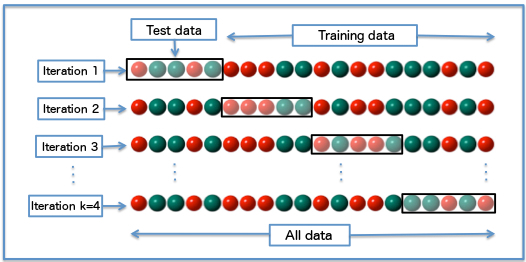
\includegraphics[width=0.6\columnwidth]{../images/K-fold_cross_validation_EN}
  \caption{4-fold cross validation on a dataset.}
\end{figure}
 
The results of our cross validation are represented in the table below. The error rates are averaged over the 5 folds.
\begin{table}[H]
  \centering
  \begin{tabular}{||c | c | c||} 
    \hline
    Algorithm & MNIST & Yale B \\
    \hline\hline
    LDA & \%  & \% \\ 
    \hline
    Decision Tree & \% & \% \\ 
    \hline
    Extra-Trees & \% (100 extra-trees) & \% (100 extra-trees) \\
    \hline
  \end{tabular}
  \caption{Average classification errors achieved with LDA, Decision Trees, and Extra-Trees after Cross Validation.}
\end{table}




%%%%%%%%%%
%%%%%%%%%%
%%%%%%%%%%
%%%%%%%%%%%%%%%%%%%%%%%%%%%%%%%%%%%%%%%%%%%%%%%%%%%%%%%%%%%%%%%%%%%%%%
% old
\iffalse
\subsection{Preliminary Hyperparameter Optimization}

\subsubsection{Decision Trees}

The table below illustrates some results that we obtained during various configurations of the decision tree training algorithm on MNIST. In an effort to optimize training time vs. test accuracy, we noticed some trends in the algorithm's performance. Notably, utilizing \code{minLeaf} doesn't seem to contribute to over-fitting, as was noted in other implementations \cite{matlab:fitctree}. This may be in part to the type of algorithm we are using. Particularly, the pure C4.5 algorithm moves back up the tree if certain conditions are met, thereby improving a previously-made split. This bore more complexity than we were able to achieve at this time, but may be responsible for a more simpler tree generation on our part. Note that for MNIST, we used half of the 70k samples for training and half for testing.

\begin{table}[H]
  \centering
  \begin{tabular}{||c | c | c | c | c | c | c | c | c | c | c | c | c ||} 
    \hline
    Training Configuration & 1 & 2 & 2 & 2 & 3 & 3 & 1 & 1 & 1 & 1 & 4 & 4 \\
    \hline
    numFeatures & 30 & 30 & 60 & 200 & 200 & 200 & 30 & 100 & 100 &  20 & 10 & 10 \\
    \hline
    minLeaf & 1 & 1 & 2 & 2 & 3 & 4 & 4 & 4 & 1 & 1 & 1 & 3 \\
    \hline
    Error Rate (\%) & 22 & 26 & 26 & 26 & 23 & 24 & 22.6 & 23.6 & 23.5 & 22.9 & 17.42 & 20.37 \\
    \hline
    Mins To Train & 48 & 2 & 2 & 3 & 12 & 12 & 47 & 60 & 102 & 11 & 3 & 3 \\
    \hline
  \end{tabular}
  \caption{Hyperparameter Configuration of Decision Tree for MNIST.}
\end{table}

The training configurations were primarily modifications to the algorithm's search through the features to find the best one to split the set on. They are as follows:

%
\begin{enumerate}
\item All features were considered for the best information gain in a particular set.
\item The decision tree was grown by considering only the first feature in the set. This was an attempt to reduce the computational complexity.
\item If the number of features left in a set was greater than 5, we considered only the first 5. Otherwise, we considered all features left. 
\item For configurations 1-3, we utilized features generated via PCA. For this experiment, we utilized features generated with LDA. This yielded our best performance.
\end{enumerate}

\fi